\nonstopmode
\documentclass{llncs}
\usepackage{graphicx}
\usepackage{verbatim}
\usepackage{amssymb}
\newcommand{\Butterfly}{\mbox{\large $\rhd\!\!\!\lhd$}}
\newcommand{\sync}[1]{\raisebox{-1.0ex}{$\;\stackrel{\Butterfly}{\scriptscriptstyle #1}\,$}}
\title{Bio-PEPA Model Report}
\author{Bio-PEPA Workbench}
\institute{\today}
\begin{document}
\maketitle
\section{Bio-PEPA model}



\begin{eqnarray*}
r_1 & = & [k_1 \times  E \times  S]\\%
r_{-1} & = & [k_{-1} \times  \hbox{\textit{E:S}}]\\%
r_2 & = & [k_2 \times  \hbox{\textit{E:S}}]\\%
%
E & = & r_1{\downarrow} +  r_{-1}{\uparrow}  +  r_2{\uparrow} \\%
S & = & r_1{\downarrow}  +  r_{-1}{\uparrow} \\%
\hbox{\textit{E:S}} & = & r_1{\uparrow}  +  r_{-1}{\downarrow}  +  r_2{\downarrow} \\%
P & = & r_2{\uparrow} \\%
\end{eqnarray*}
%
\begin{displaymath}
(E \sync{\{r_1, r_{-1}, r_2\}} (S \sync{\{r_1, r_{-1}\}} (\hbox{\textit{E:S}} \sync{\{r_2\}} P)))%
\end{displaymath}

\begin{figure}[htbp]
\begin{center}
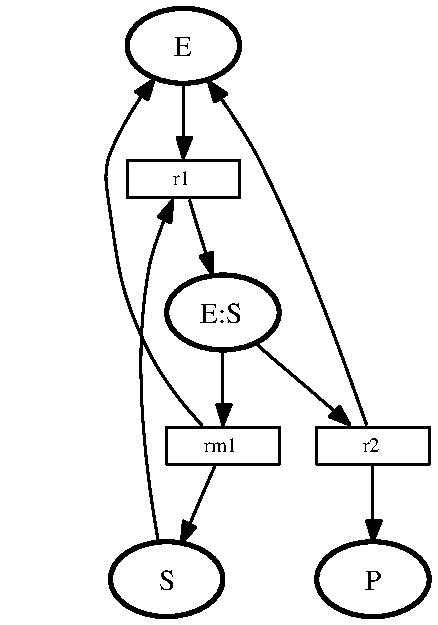
\includegraphics[width=0.6\textwidth]{dot/mm.pdf}
\caption{Reaction network}
\end{center}
\end{figure}
\newpage
\section{Graphs from Bio-PEPA model}
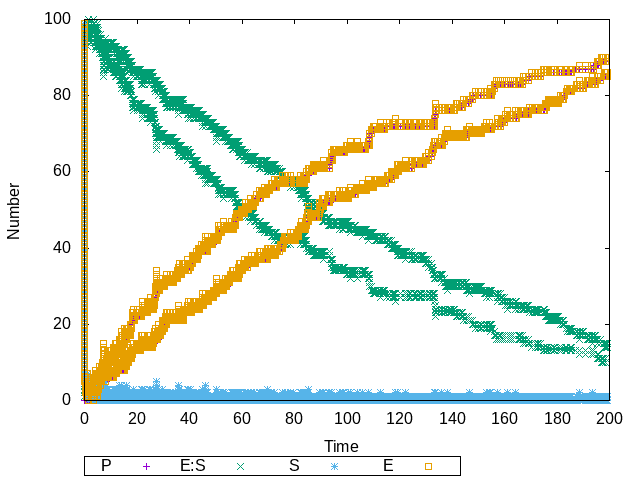
\includegraphics[scale=0.5]{png/mm001_stochkit_results_0}
\hfill
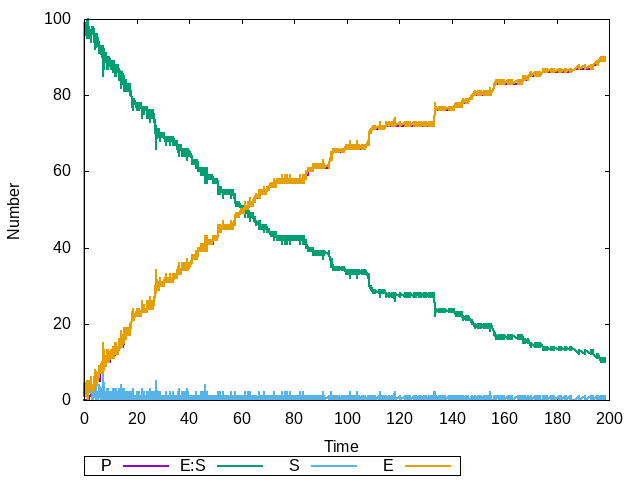
\includegraphics[scale=0.5]{png/mm001_stochkit_results_1}
\hfill
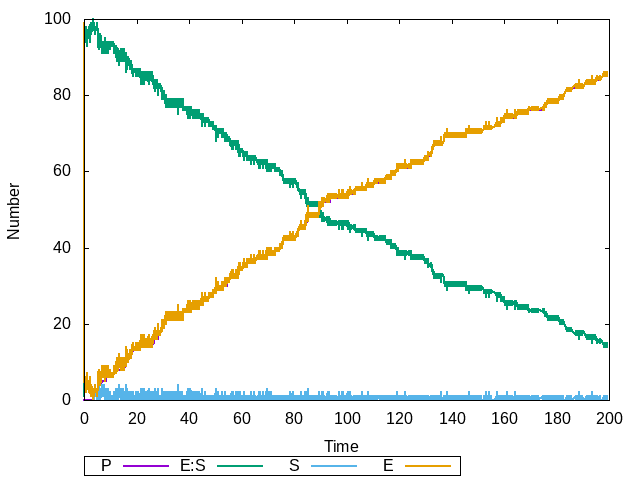
\includegraphics[scale=0.5]{png/mm001_stochkit_results_2}
\hfill
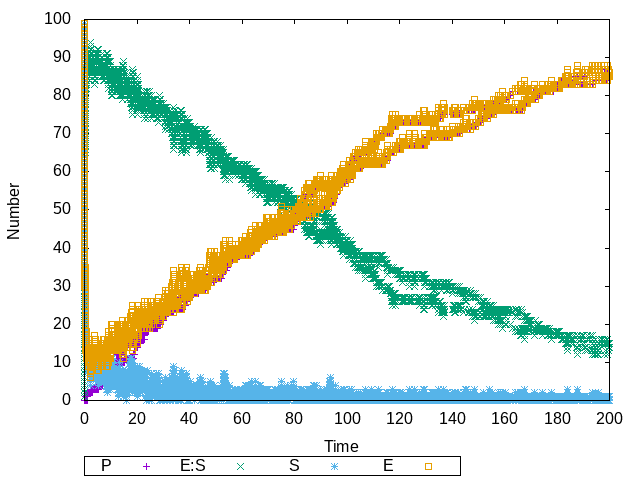
\includegraphics[scale=0.5]{png/mm002_stochkit_results_0}
\hfill
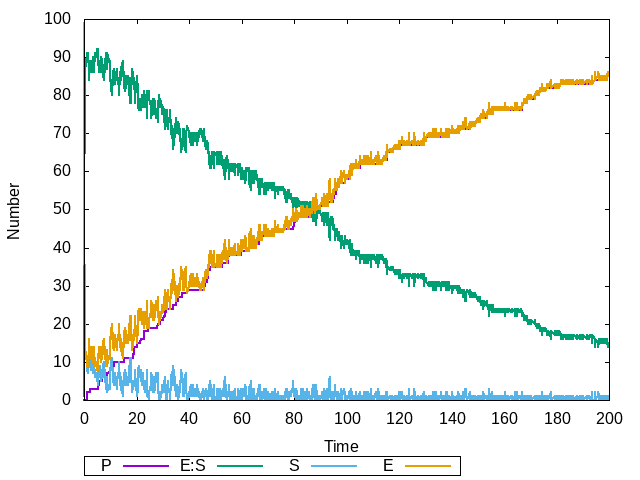
\includegraphics[scale=0.5]{png/mm002_stochkit_results_1}
\hfill
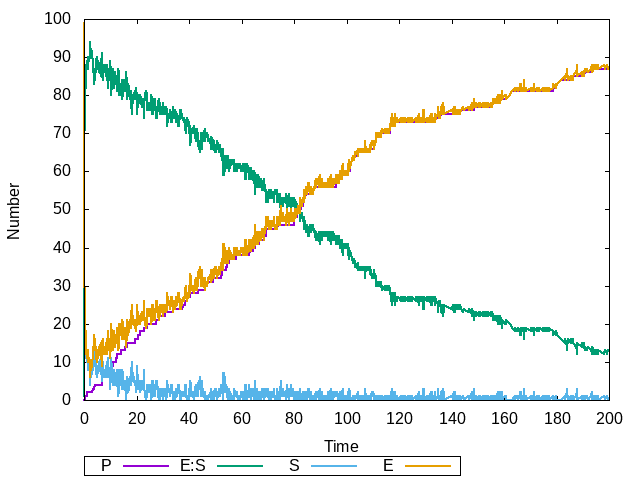
\includegraphics[scale=0.5]{png/mm002_stochkit_results_2}
\hfill
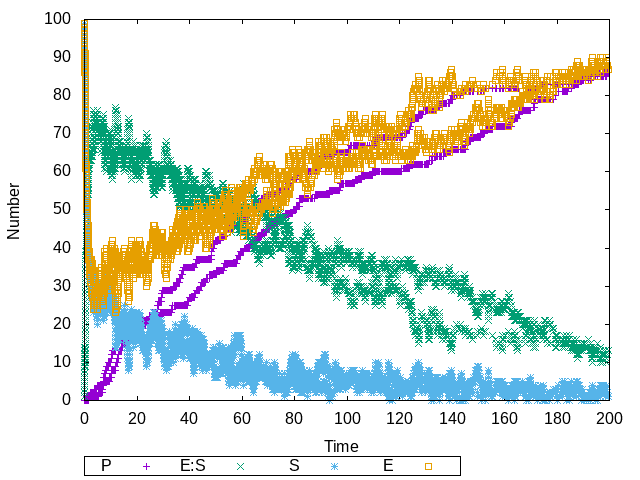
\includegraphics[scale=0.5]{png/mm003_stochkit_results_0}
\hfill
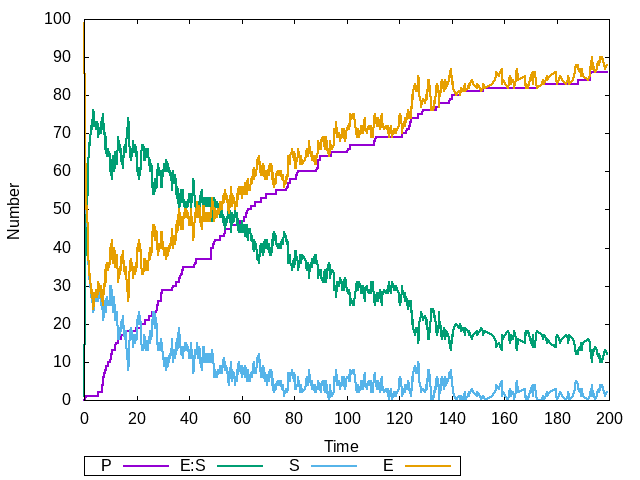
\includegraphics[scale=0.5]{png/mm003_stochkit_results_1}
\hfill
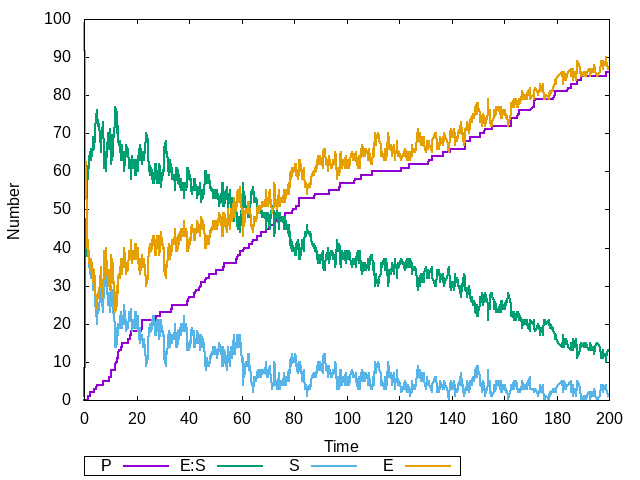
\includegraphics[scale=0.5]{png/mm003_stochkit_results_2}
\appendix
\newpage
\section{Bio-PEPA input file}
\verbatiminput{mm.biopepa}
\newpage
\section{Dizzy equivalent input file}
\verbatiminput{dizzy/mm001.dizzy}
\newpage
\section{PRISM equivalent input file}
\verbatiminput{prism/mm001.sm}
\end{document}
